\documentclass[a4paper]{article}
\usepackage[14pt]{extsizes} 
\usepackage[T2A]{fontenc}
\usepackage[utf8]{inputenc}
\usepackage{natbib}
\usepackage{graphicx}
\usepackage{amsmath}
\usepackage[english, russian]{babel}
\usepackage{fontspec}
\usepackage{amsmath,amsfonts,amssymb,amsthm,mathtools,mathrsfs}
\usepackage{icomma}
\usepackage{fullpage}
\usepackage{ulem}
\usepackage{eufrak}
\usepackage{setspace}
\usepackage{listings}
\usepackage{indentfirst}
\usepackage[left=2cm,right=1.5cm,top=2cm,bottom=2cm]{geometry}
\usepackage{xcolor}
\usepackage{float}
\usepackage{csquotes}

\setmainfont[Ligatures={TeX,Historic}]{Times New Roman}
\setlength{\parindent}{5ex}
\setlength{\parskip}{1em}
\renewcommand{\baselinestretch}{1}

\graphicspath{{images/}}

\definecolor{buzzlightyear}{HTML}{8757A5}
\definecolor{grass}{HTML}{738D06}
\definecolor{literal}{HTML}{F18A2B}
\definecolor{commentcolor}{HTML}{8E908B}

\lstdefinestyle{habrstyle}{
    backgroundcolor=\color{white},   
    commentstyle=\color{commentcolor},
    keywordstyle=\bfseries\color{buzzlightyear},
    numberstyle=\tiny\color{commentcolor},
    stringstyle=\color{grass},
    basicstyle=\ttfamily\footnotesize,
    breakatwhitespace=false,         
    breaklines=true,                 
    captionpos=b,                    
    keepspaces=true,                 
    numbers=left,                    
    numbersep=5pt,                  
    showspaces=false,                
    showstringspaces=false,
    showtabs=false,                  
    tabsize=4
}

\lstset{style=habrstyle}

\begin{document}
    % НАЧАЛО ТИТУЛЬНОГО ЛИСТА
    \begin{center}
        \begin{center}
        \hfill \break
        \normalsize{Санкт-Петербургский государственный политехнический}\\
        \normalsize{университет Петра Великого}\\
        \hfill \break
        \normalsize{\textbf{Высшая школа интеллектуальных систем и}}\\ 
        \normalsize{\textbf{суперкомпьютерных технологий}}\\ 
        \hfill \break
        \hfill \break
        \hfill \break
        \normalsize{Лабораторная работа}\\
        \hfill \break
        \hfill \break
        \normalsize{\LARGE Линейные стационарные системы}\\
        \end{center}
        \hfill \break
        \hfill \break
        \hfill \break
        \hfill \break
        \hfill \break
        \hfill \break
        \hfill \break
        \hfill \break
        \hfill \break
        \hfill \break
        \begin{flushright}
            \normalsize{Работу выполнил студент}\\
            \normalsize{3-го курса, группа 3530901/80201}\\
            \normalsize{Солянкин Илья Андреевич}\\
            \hfill \break
            \normalsize{Преподаватель:}\\
            \normalsize{Богач Наталья Владимировна}\\
        \end{flushright}
        \hfill \break
        \hfill \break
        \hfill \break
        \hfill \break
        \begin{center} Санкт-Петербург 2021 \end{center}
        \thispagestyle{empty}
    \end{center}
    % КОНЕЦ ТИТУЛЬНОГО ЛИСТА
    
    % ОГЛАВЛЕНИЕ
    \newpage
        \tableofcontents
    
    % СПИСОК ИЛЛЮСТРАЦИЙ
    \newpage
         \listoffigures
    
    % СПИСОК ЛИСТИНГОВ     
    \newpage
         \lstlistoflistings   
     
    \newpage
        \section{Часть №1: \texttt{chap10.ipynb}}
            В первой части десятой лабораторной работы нам необходимо просмотреть весь блокнот \texttt{chap10.ipynb}, после чего заменить его, чтобы устранить лишнюю ноту в начале фрагмента.
            
            Возмем исходный сигнал и выведем его на экран:
            
\begin{lstlisting}[language=Python, caption= Получение сигнала]
    response = read_wave('180960__kleeb__gunshot.wav')
    start = 0.12
    response = response.segment(start=start)
    response.shift(-start)
    
    response.truncate(2**16)
    response.zero_pad(2**17)
    
    response.normalize()
    response.plot()
    decorate(xlabel='Time (s)')
\end{lstlisting}
            
            \begin{figure}[H]
                \centering
                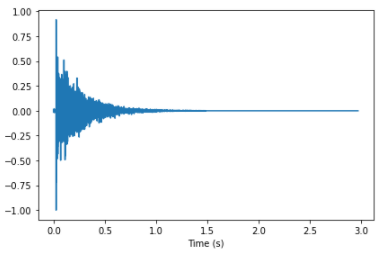
\includegraphics{ex_1_1.png}
                \caption{Начальный сигнал}
                \label{fig:ex_1_1}
            \end{figure}
            
            После этого получим спектр данного сигнала:
            
\begin{lstlisting}[language=Python, caption= Получение спектра первого сигнала]
    transfer = response.make_spectrum()
    transfer.plot()
    decorate(xlabel='Frequency (Hz)', ylabel='Amplitude')
\end{lstlisting}
            
            \begin{figure}[H]
                \centering
                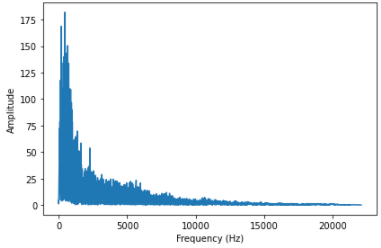
\includegraphics{ex_1_2.png}
                \caption{Спектр первого сигнала}
                \label{fig:ex_1_2}
            \end{figure}
            
            Теперь возьмем второй сигнал со скрипкой:
            
\begin{lstlisting}[language=Python, caption= Получение второго сигнала]
    violin = read_wave('92002__jcveliz__violin-origional.wav')

    start = 0.11
    violin = violin.segment(start=start)
    violin.shift(-start)
    
    violin.truncate(2**16)
    violin.zero_pad(2**17)
    
    violin.normalize()
    violin.plot()
    decorate(xlabel='Time (s)')
\end{lstlisting}
            
            \begin{figure}[H]
                \centering
                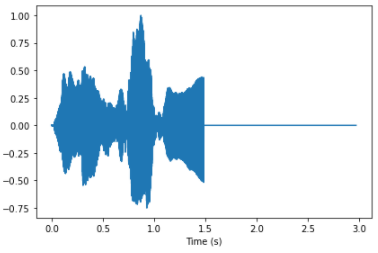
\includegraphics{ex_1_3.png}
                \caption{Начальный второй спектр}
                \label{fig:ex_1_3}
            \end{figure}
            
            И так же получим для его спектр:
            
\begin{lstlisting}[language=Python, caption= Получение спектра второго сигнала]
    spectrum = violin.make_spectrum()
    spectrum.plot()
\end{lstlisting}
            
            \begin{figure}[H]
                \centering
                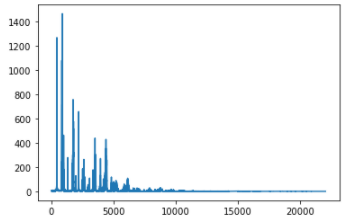
\includegraphics{ex_1_4.png}
                \caption{Спектр второго сигнала}
                \label{fig:ex_1_4}
            \end{figure}
            
            После этого усножим ДПФ сигнала на передаточную функцию, после чего преобразуем обратно в волну и выведем полученный сигнал на экран:
            
\begin{lstlisting}[language=Python, caption= Преобразование сигнала]
    output = (spectrum * transfer).make_wave()
    output.normalize()
    output.plot()
\end{lstlisting}
            
            \begin{figure}[H]
                \centering
                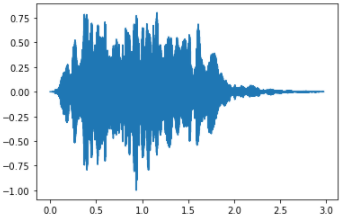
\includegraphics{ex_1_5.png}
                \caption{Полученный сигнал}
                \label{fig:ex_1_5}
            \end{figure}
            
            Нам осталось представить полученный сигнал в виде аудио и сравнить его с изначальным:
            
            \begin{figure}[H]
                \centering
                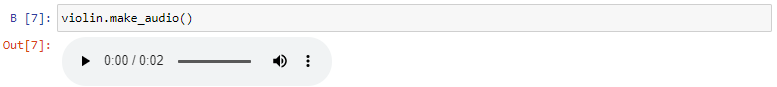
\includegraphics[width=\textwidth]{ex_1_6.png}
                \caption{Изначальный сигнал}
                \label{fig:ex_1_6}
            \end{figure}
            
            \begin{figure}[H]
                \centering
                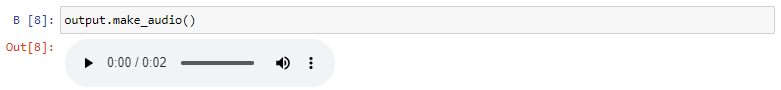
\includegraphics[width=\textwidth]{ex_1_7.png}
                \caption{Полученный сигнал}
                \label{fig:ex_1_7}
            \end{figure}
            
            В ходе сравнения стало понятно, что исчезла нота, стоящая в начале фрагмента.
            
    \newpage
        \section{Часть №2: Изменение звучания сигнала}
            Во втором пункте десятой лабораторной работы нам необходимо  смоделировать двумя способами звучание записи в том пространстве, где была измерена импульсная характеристика, как сверткой самой записи с импульсивной зарактеристикой, так и умножением ДПФ записи на вычислительный фильтр.
            
            Скачаем файл со звуком лопнувшего шарика и сразу выведем его на экран:
            
\begin{lstlisting}[language=Python, caption= Получение сигнала]
    response = read_wave('balloon2.wav')

    start = 0
    duration = 1
    response = response.segment(duration=duration)
    response.shift(-start)
    
    response.normalize()
    response.plot()
    decorate(xlabel='Time (s)')
\end{lstlisting}
            
            \begin{figure}[H]
                \centering
                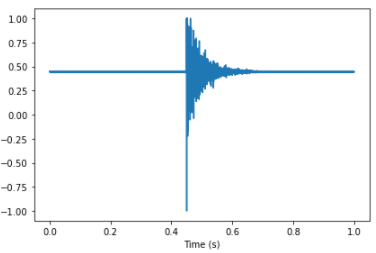
\includegraphics{ex_2_1.png}
                \caption{Полученный сигнал}
                \label{fig:ex_2_1}
            \end{figure}
            
            Теперь получим спектр данного сигнала:
            
\begin{lstlisting}[language=Python, caption= Получение спектра сигнала]
    transfer = response.make_spectrum()
    transfer.plot()
    decorate(xlabel='Frequency (Hz)', ylabel='Amplitude')
\end{lstlisting}
            
            \begin{figure}[H]
                \centering
                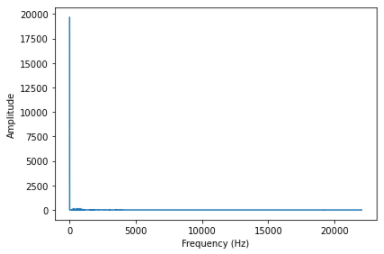
\includegraphics{ex_2_2.png}
                \caption{Спектр сигнала}
                \label{fig:ex_2_2}
            \end{figure}
            
            И, наконец, представим его в логарифмическом масштабе:
            
\begin{lstlisting}[language=Python, caption= Получение спектра сигнала в логарифмическом масштабе]
    transfer.plot()
    decorate(xlabel='Frequency (Hz)', ylabel='Amplitude', xscale='log', yscale='log')
\end{lstlisting}
            
            \begin{figure}[H]
                \centering
                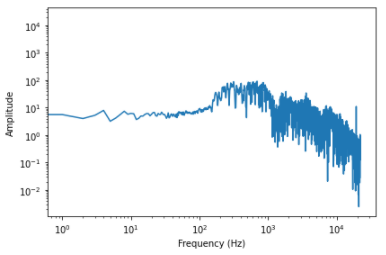
\includegraphics{ex_2_3.png}
                \caption{Спектр сигнала в логарифмическом масштабе}
                \label{fig:ex_2_3}
            \end{figure}
            
            Также можно смоделировать звучание записи, если она будет воспроизводиться в одной комнате.
            
            Для этого вычислим ДПФ использованной в прошлом пункте записи скрипки:
            
\begin{lstlisting}[language=Python, caption= Получение сигнала скрипки]
    wave = read_wave('92002__jcveliz__violin-origional.wav')
    
    start = 0.0
    wave = wave.segment(start=start)
    wave.shift(-start)
    
    wave.truncate(len(response))
    wave.normalize()
    wave.plot()
    decorate(xlabel='Time (s)')
\end{lstlisting}
            
            \begin{figure}[H]
                \centering
                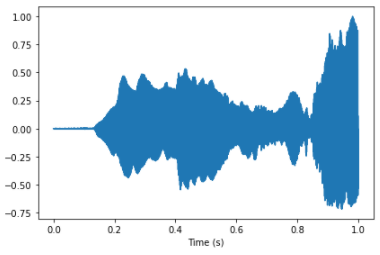
\includegraphics{ex_2_4.png}
                \caption{Полученный сигнал скрипки}
                \label{fig:ex_2_4}
            \end{figure}
            
            Теперь ображем запись скрипки до той же длины, что и испульсная характеристика:
            
            \begin{figure}[H]
                \centering
                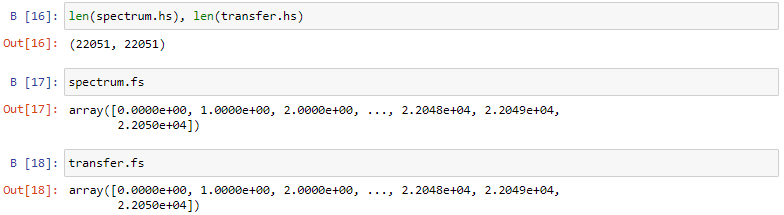
\includegraphics[width=\textwidth]{ex_2_5.png}
                \caption{Обрезание записи скрипки}
                \label{fig:ex_2_5}
            \end{figure}
            
            После этого выполним умножение в частотной области и преобразуем обратно во временную область, после чего выведем полученный результат на экран:
            
\begin{lstlisting}[language=Python, caption= Получение результата]
    output = (spectrum * transfer).make_wave()
    output.normalize()
    output.plot()
\end{lstlisting}
            
            \begin{figure}[H]
                \centering
                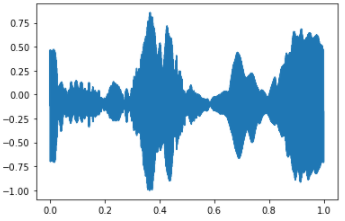
\includegraphics{ex_2_6.png}
                \caption{Полученный результат}
                \label{fig:ex_2_6}
            \end{figure}
            
            Теперь нам осталось только представить полученный сигнал в виде аудио, после чего воспользуемся методом \texttt{convolve} для свертки:
            
            \begin{figure}[H]
                \centering
                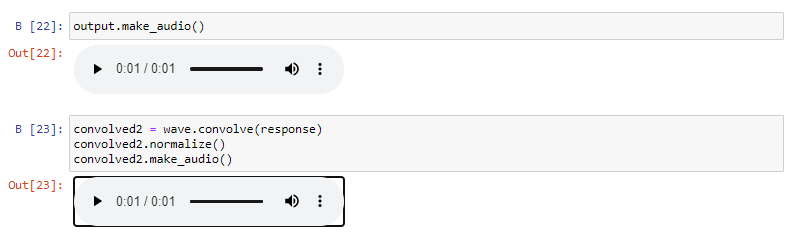
\includegraphics[width=\textwidth]{ex_2_7.png}
                \caption{Сравнение результата с иходной записью}
                \label{fig:ex_2_7}
            \end{figure}
            
            В результате выполнения данного пункта мы получили чистый и довольно реалистичный звук игры на скрипке внутри помещения.
            
    \newpage
        \section{Выводы}
             В результате выполнения данной лабораторной работы нами были получены знания о свертке сигналов. Нами была модифицирована запись игры на скрипке, в которой была убрана первая нота. Кроме того мы смоделировали звучание записи в помещении.
            
\end{document}
